% Generated by pysimcount.pffigure -- do not edit; regenerate instead.
% figure: C-lie-trotter-by-bound -- Lie-Trotter S1: r from each bound and measured
% source: results/pf-thesis/results.json
% metric=t gatebase=ct merged
% seed=1 t=n template=simcount synth=pygridsynth
% git_commit=04cd66abb614bdc66fb48e891cef085a299e0ab1 git_dirty=False
% source_sha256=018e0b7603e6fc9f6ee358974f241415a3b93437700847b033937cc1d4250db8
% derived: C-lie-trotter-by-bound.tex restyled by pysimcount.figuniform: extrapolated points (r from power-law fit) drawn in their series' measured style, style-key legend entries removed; extrapolated n = [13, 20]; source_sha256=8b8b18961f2fcf3e69f4e1e27f4e700b01b8985cb07a0d9f5a7be63c6841563d
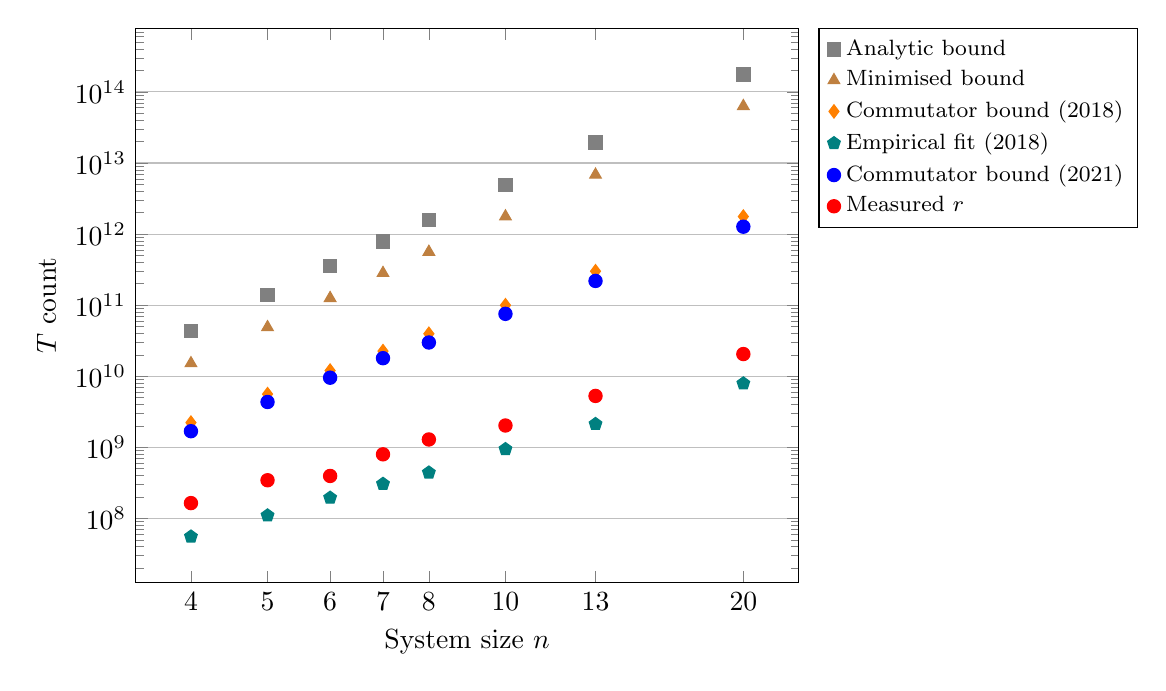
\begin{tikzpicture}
  \begin{loglogaxis}[
    width=10cm,
    xlabel={System size $n$},
    ylabel={$T$ count},
    xtick={4,5,6,7,8,10,13,20},
    xticklabels={4,5,6,7,8,10,13,20},
    ymajorgrids=true,
    legend pos=outer north east,
    legend cell align=left,
    legend style={font=\footnotesize},
  ]
    \addplot[only marks, gray, mark=square*, mark size=2.4pt, mark options={solid, fill=gray}] coordinates {
      (4,43556530740)
      (5,138958568172)
      (6,356234965440)
      (7,783609064560)
      (8,1571954286032)
      (10,4897256547180)
      (13,19378157089200)
      (20,176336029528540)
    };
    \addlegendentry{Analytic bound}
    \addplot[only marks, brown, mark=triangle*, mark size=2.4pt, mark options={solid, fill=brown}] coordinates {
      (4,15204470784)
      (5,48880244400)
      (6,125494707744)
      (7,282588816888)
      (8,561775689216)
      (10,1768322210400)
      (13,6838193921832)
      (20,63098899718400)
    };
    \addlegendentry{Minimised bound}
    \addplot[only marks, orange, mark=diamond*, mark size=2.4pt, mark options={solid, fill=orange}] coordinates {
      (4,2224878106)
      (5,5605598614)
      (6,12019522502)
      (7,22585529744)
      (8,39551101166)
      (10,99690635856)
      (13,300317990958)
      (20,1765948340376)
    };
    \addlegendentry{Commutator bound (2018)}
    \addplot[only marks, teal, mark=pentagon*, mark size=2.4pt, mark options={solid, fill=teal}] coordinates {
      (4,55411764)
      (5,109839780)
      (6,194992930)
      (7,305460444)
      (8,440979456)
      (10,941620000)
      (13,2123198700)
      (20,7909890288)
    };
    \addlegendentry{Empirical fit (2018)}
    \addplot[only marks, blue, mark=oplus*, mark size=2.4pt, mark options={solid, fill=blue}] coordinates {
      (4,1685202624)
      (5,4342683520)
      (6,9543017998)
      (7,17942187654)
      (8,29832119562)
      (10,75470365476)
      (13,219200151920)
      (20,1270851259104)
    };
    \addlegendentry{Commutator bound (2021)}
    \addplot[only marks, red, mark=*, mark size=2.4pt, mark options={solid, fill=red}] coordinates {
      (4,164071520)
      (5,343961840)
      (6,395184006)
      (7,797117356)
      (8,1288997320)
      (10,2026934136)
    };
    \addlegendentry{Measured $r$}
    % r from power-law fit (extrapolation); one legend entry per series
    \addplot[only marks, red, mark=*, mark size=2.4pt, mark options={solid, fill=red}, forget plot] coordinates {
      (13,5281447392)
      (20,20514256040)
    };
  \end{loglogaxis}
\end{tikzpicture}
